
\subsection*{EE Stuff}
\begin{tabular}{ll}
Norton&$I_{sc} || R_{oc}$\\

Thevenin&$V_{oc} + R_{sc}$\\

Max power &$R_L = R_{thevenin}$\\

NVA$\rightarrow$KCL$\rightarrow$& $\dfrac{v_{ab}}{R_1} + \dfrac{v_{ac}}{R_2} +
\cdots = 0$\\

MCA$\rightarrow$KVL$\rightarrow$& $R_1i_1 + R_2i_2 + \cdots = 0$\\
\end{tabular}

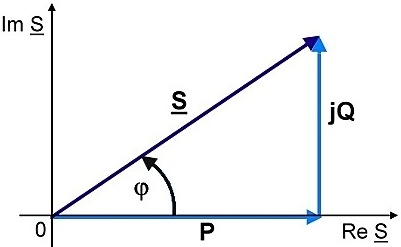
\includegraphics[width=40mm]{ACPower.jpg}
\begin{tabular}{cc}
real \textbar{} reactive & R \textbar{} Q\\
complex  apparent& S \textbar S\textbar\\
power factor & $\cos \psi$\\
$ \jmath \omega L = $&$ Z_L$\\
$\dfrac{-\jmath}{\omega C} = \dfrac{1}{\jmath \omega C} = $&$Z_c$\\
\end{tabular}
\vfill
\[
A_{v/i} = 20 \log_{10}{|A_{v/i}|} dB \hspace{15 mm} A_p = 10 log|A_p| dB
\]
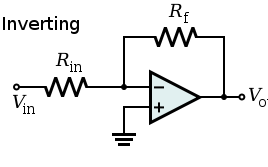
\includegraphics[width=60mm]{inverting-amp.png} 

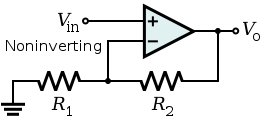
\includegraphics[width=60mm]{noninverting-amp.png} 
\vfill
Differential input is $v_1 - v_2$ Common mode input is $\dfrac{v_1+v_2}{2}$

Amplifier Types: V,I, Transconductance ($G_m=\dfrac{i_o}{v_i}$),
Transresistance ($R_m=\dfrac{v_o}{i_i}$)

Ideal Inputs and Outputs: 
\begin{tabular}{ccc}
i&$R_i=0$&$R_o=\infty$\\
v&$R_i=\infty$&$R_o=0$\\
\end{tabular}
%\subsubsection*{Diode Models}
%\begin{description}
%\item[Constant voltage drop] ideal + $v_{DD} = 0.7$
%\item[Piecewise linear] (ideal + $v_{DD} + r_D$) slope is $\frac{1}{r_D}$
%\item[small signal] slope $=\frac{1}{r_D}$ where $r_d = \frac{n V_T}{I_D}$ and
%$i_D = \frac{v_d}{r_d}$ \end{description}
\subsubsection*{2104 Odds and Ends}

\begin{tabular}{cl}
half wave&$\tau= RC$\\
$V_r = V_p \dfrac{T}{\tau} = V_p\dfrac{1}{f\tau }$&$v_r$ is v drop\\
full wave&$T$ is discharge time\\
$V_r = \dfrac{V_p}{2f\tau }$&f \mbox{ is the supply freq}\\
new freq is&$2f$\\
\end{tabular}
% \mbox{ new freq}\]

\vfill

\[
\begin{array}{ccc}
Line    &   Load    &   Voltage\\
\dfrac{\Delta V_O}{ \Delta V_s} &\dfrac{\Delta V_O }{\Delta I_L }&\dfrac{V_{NL}
- V_{FL}}{V_{NL}}\\

\mbox{ s = source} & \mbox{O = output}&\Delta \mbox{ = percentage}\\
\end{array}
\]
\vfill
BJT... \emph{current flows in direction of arrow}
\[ 
\begin{array}{cc}
I_E = I_C + I_B&\mbox{pnp }=  E \rightarrow B\\
\alpha = \frac{I_C}{I_E}& \beta = \frac{I_C}{I_B}\\
\alpha = \dfrac{\beta}{\beta + 1}&\\
\end{array}
\]
\vfill
Hybrid $\pi$ model. Add resistor $r_0$ in parallel to $I$ source for Early effect.
\[ 
\begin{array}{cc}
v_\pi = v_{BE}&r_\pi = r_{BE}\\
i_{C} = \beta i_b = g_m v_\pi&\\
\end{array}
\]
T Model has 
\[i_c = g_m v_{be} = \alpha i_e \mbox{ and }v_{be} = i_e r_e\]
Relating the T model and hybrid $\pi$ model.
\[ r_\pi = (\beta + 1 )r_e\]
MOSFET \ \ \ \ \emph{ where} $\beta$ always = $\infty$
\medskip

When $v_{GS} \ge V_t$ the channel is conductive. 
\smallskip

$L$ is length between $S$ and $D$ doped (0.1-3$\mu$m). 
\smallskip

$W$ is width of device (0.2-100$\mu$m).
\smallskip

$k^\prime_n$ is the transconductance $\left(\dfrac{A}{V^2}\right)$.

NMOS has n gates and P substrate. PMOS has p gates and N substrate (usually an
N well in P substrate). We ignore the voltage of the body (B).

Polarity of voltage determines which side is source or drain. Drain is
\emph{always positive relative to source in n-channel MOSFET}. Arrow is at
source end. Points to source in n-channel, away in p-channel.

Triode region is where $v_{DS} \le v_{GS} - V_t$

\subsubsection*{2104 Formulae}
BJT Equations
\[
\begin{array}{cc}
i_c = I_S e^{v_{BE}/V_T}    & g_m = \dfrac{I_C}{V_T}\\
r_e = \dfrac{V_T}{I_E}       &r_o = \dfrac{V_A}{I_C}
\end{array}
\]
MOSFET equations
\[ i_D = \frac{1}{2} k_n^\prime \frac{W}{L}(v_{GS} - V_t)^2 = k(v_{GS} -
V_t)^2\]

\[g_m = k_n^\prime \frac{W}{L} (V_{GS} - V_t) = \frac{2i_D}{(V_{GS} - v_t)}\]
JFET equations
\[i_D = I_{DSS} \left(1 - \frac{V_{GS}}{V_P}\right)^2\]
\[g_m = \left(\frac{2I_{DSS}}{|V_p|}\right)\sqrt{\frac{I_D}{I{DSS}}}\]

%\subsubsection*{3405 Stuff}
%Gain of a feedback amp:
%\[ A = \dfrac{x_0}{x_i}=\dfrac{a}{1+a\cdot \beta}\]

\subsubsection*{3404 Formulae}
\[ \begin{array}{cccc}
r_0=  &     &g_m    &\\
r_\pi &     &\alpha &\\
r_e   &     &f_t    &\\
\end{array} \]
\emph{Formulae you should know...}
\[ \begin{array}{rlrl}
P_S=&2I_SV_{CC}=\dfrac{2V_{CC}\hat{V}_O}{\pi R_L}&
P_L=&\dfrac{\hat{V}^2_O}{2 R_L}\\
\hat{V}_O|_{P_{Dmax}}=&\dfrac{2 V_{CC}}{\pi}
&P_{Dmax}=&\dfrac{2V^2_{CC}}{\pi^2R_L}\\
f_L=&f_{L1}+f_{L2}+f_{L3}&f_H=&\dfrac{1}{2\pi C_{in}R'_{sig}}\\
C_{in}= &C_\pi+C_{eq}&&\\
        &C_\pi+C_\mu(1+g_mR'_L)&&\\
\end{array}\]
In HF hybrid $\pi$-model $C_\pi||r_\pi$ and $C_\mu$ connects base and collector.

$f_L$ and $f_H$ are the lower and upper 3dB frequencies.
\columnbreak
\subsubsection*{Signals and Systems}
Unilateral laplace properties \[x \rightarrow x(t) \mbox{ and } X \rightarrow X(s)\]

\begin{tabular}{crcll}
linearity& $a_1x_1 + a_2x_2i$&$\leftrightarrow $&$a_1X_1+a_2X_2$&\\
time shift& $x(t-t+0) $&$\leftrightarrow $&$X(s)e^{-t_0s}$ & $t_0 > 0$\\
time scale&$x(at)$&$ \leftrightarrow $&$X\left( \frac{s}{a} \right)$ & $a>0$\\
cplx shif& $e^{-at}x $&$\leftrightarrow $&$X(s+a)$&\\
conv& $x(t)*h(t) $&$\leftrightarrow $&$X(s)H(s)$&\\
\end{tabular}

\[Y(s) = X(s)\left[ \frac{A(s)}{1+A(s) \beta (s)}\right] \]
Some Transforms
\[
\begin{array}{cc}
d{t}&1\\
u(t)&\dfrac{1}{s}\\
t^n e^{\lambda t} u{t}& \dfrac{n!}{(s - \lambda)^{n+1}}\\
e^{-at}\cos{(bt)}u(t)& \dfrac{s+a}{(s+a)^2 + b^2}\\
e^{-at}\sin{(bt)}u(t)& \dfrac{b}{(s+a)^2 + b^2}\\
\end{array}
\]

Differentiation in time
\[
\begin{array}{l}
\frac{\partial^n x(t)}{\partial t^n} \leftrightarrow s^nX(s) - \\
\left(s^{n-1} x(0^-) + s^{n-2}\left[\frac{\partial x(t)}{\partial
t}\right]_{t=0^-}+ \ldots + \left[\frac{\partial^{n-1}x(t)}{\partial t^{n-1}}
\right]_{t=0^-}\right) \end{array}
\]
for example \ldots 
\[\frac{\partial x(t)}{\partial t} \leftrightarrow sX(s) - x(0^-)\]
\[t^nx(t) \leftrightarrow (-1)^n \frac{\partial^nX(s)}{\partial x^n}\]

Integration in time
\[
\int^t_{0} x(\tau) d\tau \leftrightarrow \frac{1}{s}X(s) +  x(0^-)
\]
\begin{tabular}{cccc}
IVT&$x(0^+)$&=&$\lim_{s \to \infty} sX(s)$\\
FVT&$\lim_{t\to \infty} x(t)$&=&$\lim_{s\to \infty} sX(s)$
\end{tabular}

\clearpage
\subsection*{Communications}
The OSI model

\begin{tabular}{cll}
&layer&examples\\
7&application&http nfs ftp\\
6&presentation&MIME SSL\\
5&session&\\
4&transport&TCP UDP\\
3&network&IPv4 ICMP\\
2&data link control&PPP DHCP\\
1&physical&802.11 802.3\\
\end{tabular}

Elements of a Digital System

\begin{tabular}{cc}
information&\\
&(message signal)\\
source encodeer&\\
&(source codeword)\\
channel encoder&\\
&(channel codeword)\\
digital modulator&\\
&(waveform)\\
channel&\\
\end{tabular}

\subsubsection*{Shannon's information capacity theorem}

Constraints (power, bandwidth, cost)

Reliability is measured by Bit Error Rate (BER)
\[
C = B \log_2 (1+SNR) \mbox{ \ \ bits per second}
\]
\begin{tabular}{llll}
C&information capacity&B& channel BW\\
R& signaling rate&SNR& s / n ratio\\
W& message BW\\
\end{tabular}
\[
\eta = \frac{R}{C} \mbox{ \ \ measure of system efficiency}
\]

\subsubsection*{Continuous Wave Modulation}
\textbf{AM}
\begin{align*}
c(t) &=A_c \cos (2\pi f_ct)& \mbox{ carrier}\\
m(t) &  &\mbox{bband sig}\\
s(t) &=A_c \cos \left[1+K_am(t)\right] \cos(2\pi f_ct) &\mbox{modulated}\\
\end{align*}

Envelope of s(t) has the same shape as m(t) for $|K_a m(t)| < 1$ and $f_c >> W$

Fourier Transfom:
\[S(f) = 1/2 A_c [\delta(f-f_c)+\delta(f+f_c)]\]
\[+ 1/2K_aA_c[M(f-f_c)+M(f+fc)]\]


\begin{description}
\item[] Linear modulation techniques
\item[DSB-SC] $s_l(t) = m(t) , s_Q(t) = 0$
\item[SSB-LSB] $s_l(t) = 1/2 m(t) , s_Q(t) = 1/2\hat m(t)$
\item[SSB-USB]$s_l(t) = 1/2 m(t) , s_Q(t) = - 1/2\hat m(t)$
\item[VSB] vestigial sideband
\item[vestige of lsb]$s_l(t) = 1/2 m(t) , s_Q(t) =  1/2m'(t)$
\item[vestige of usb]$s_l(t) = 1/2 m(t) , s_Q(t) = - 1/2m'(t)$
\item[$m'$] output of filter of freq response of $H_Q(f)$
\item[$\hat m$] hilbert transform of $m(t)$
\end{description}

\textbf{Double Sideband - Suppressed Carrier (DSB-SC)}
\[s(t) = A_c m(t) cos(2\pi f_c t)\]
\[S(f) = \frac{A_c}{2}[M(f-f_c)+M(f+f_c)]\]
Required bandwidth = 2W
Spectrum  /\textbackslash \_\_ \textbar \_\_/\textbackslash

\[v_0(t) = 1/2 A_cA'_c \cos \phi m(t)\]
To be proportional $\phi$ is constant, using `quadrature null effect' of a
coherent detector we can send two independant message signals over the same
channel (90\textdegree out of phase).

\textbf{Single Sideband modulation}
Use a filter to remove other sideband, the message spectrum must have an
\emph{energy gap} centred at the origin.


\begin{description}
\item[Angle Modulation - PM and FM] Angle modulated signal: $s(t) = A_c
cos[\theta_i(t)]$ where $\theta_t=$ is the angle of a modulated carrier.
\item[modulating process]
\item[FM] integrator then phase modulator
\item[PM] differentiator then frequency modulator
\item Zero crossings of PM/FM are not regular. 
\item FM and PM signals have constant envelope.
\item we only discuss FM
\item[PM] $\theta_i(t) = t\pi f_ct + k_p m(t)$
\item[$k_p$] phase sensitivity constant
\item[thus] $s(t) = A_c cos[2\pi f_ct + k_pm(t)]$
\item[FM] $f_i(t) = f_c + k_f m(t)=f_c+\Delta f \cos (2\pi f_m t)$
\item[$\Delta f = k_f A_m$] frequency deviation
\item[$k_f$] frequency sensitivity constant
\item[thus] $s(t) = A_c cos[2\pi f_ct + 2\pi k_f\int^t_0m(\tau)d\tau]$
\item[$\beta = \Delta f / f_m$] modulation index
\item[narrowband FM] $\beta <<1$ radian, not ideal
\item[wideband FM] $\beta >>1$ radian
\item[power] envelope of FM is constant and avg power is $P=1/2 A_c^2$
\item FM signals have $\infty$ side freqs $\rightarrow \infty$ BW
\item[in practice] for large $\beta$ BW is slightly greater than $2\Delta f$
\item[Carson's rule] for BW of FM $B_T \approx 2\Delta f + 2f_m = 2\Delta
f(1+1/\beta)$

\item[Nonlinearity] of FM: FM is not afffected by distortion, but is
\emph{extremely sensitive} to phase non-linearity.

\item[AWGN] additive white gaussian noise
\item[BP filter] in reciever
\item[$N_0/2$] power spectral density of noise $w(t)$ for pos and neg freqs 
\item[$N_0$] avg noise power per unit bandwidth measured at front end of
reciever 
\end{description}

\subsubsection*{Pulse Modulation}
\emph{Sampling theorem:} A band-limited signal $(-W < f < W)$ of finite E is
completely described by its samples at freq 2W (Nyquist rate).

Pulse-amplitude modulation (PAM) can be multiplexed by interleaving N samples
for N signals.

We can also modulate the \emph{duration} (PDM) or \emph{position} (PPM).

Pulse-code modulation (PCM), line coding schemes: unipolar NRZ, polar NRZ,
unipolar RZ, bipolar RZ, split-phase (Manchester) or differential encoding.
Two noise sources, \emph{channel} and \emph{quantization}. We measure the
average probability of symbol errors in the recieved signal or bit-error rate
(BER).

Noise is AWGN thus BER depends on transmitted signal energy per bit and the
noise spectral density, $\dfrac{E_b}{N_0}$. Below the error threshold the
probability of an error increases sharply.

%\subsubsection*{Pulse Modulation}
%\begin{description}

%\end{description}

\clearpage

